\documentclass[11pt]{article}

    \usepackage[breakable]{tcolorbox}
    \usepackage{parskip} % Stop auto-indenting (to mimic markdown behaviour)
    

    % Basic figure setup, for now with no caption control since it's done
    % automatically by Pandoc (which extracts ![](path) syntax from Markdown).
    \usepackage{graphicx}
    % Keep aspect ratio if custom image width or height is specified
    \setkeys{Gin}{keepaspectratio}
    % Maintain compatibility with old templates. Remove in nbconvert 6.0
    \let\Oldincludegraphics\includegraphics
    % Ensure that by default, figures have no caption (until we provide a
    % proper Figure object with a Caption API and a way to capture that
    % in the conversion process - todo).
    \usepackage{caption}
    % \DeclareCaptionFormat{nocaption}{}
    % \captionsetup{format=nocaption,aboveskip=0pt,belowskip=0pt}

    \usepackage{float}
    \floatplacement{figure}{H} % forces figures to be placed at the correct location
    \usepackage{xcolor} % Allow colors to be defined
    \usepackage{enumerate} % Needed for markdown enumerations to work
    \usepackage{geometry} % Used to adjust the document margins
    \usepackage[fleqn]{amsmath} % Equations
    \usepackage{amssymb} % Equations
    \usepackage{textcomp} % defines textquotesingle
    % Hack from http://tex.stackexchange.com/a/47451/13684:
    \AtBeginDocument{%
        \def\PYZsq{\textquotesingle}% Upright quotes in Pygmentized code
    }
    \usepackage{upquote} % Upright quotes for verbatim code
    \usepackage{eurosym} % defines \euro

    \usepackage{fancyvrb} % verbatim replacement that allows latex
    \usepackage{grffile} % extends the file name processing of package graphics
                         % to support a larger range
    \makeatletter % fix for old versions of grffile with XeLaTeX
    \@ifpackagelater{grffile}{2019/11/01}
    {
      % Do nothing on new versions
    }
    {
      \def\Gread@@xetex#1{%
        \IfFileExists{"\Gin@base".bb}%
        {\Gread@eps{\Gin@base.bb}}%
        {\Gread@@xetex@aux#1}%
      }
    }
    \makeatother
    \usepackage[Export]{adjustbox} % Used to constrain images to a maximum size
    \adjustboxset{max size={0.9\linewidth}{0.9\paperheight}}

    % The hyperref package gives us a pdf with properly built
    % internal navigation ('pdf bookmarks' for the table of contents,
    % internal cross-reference links, web links for URLs, etc.)
    \usepackage{hyperref}
    % The default LaTeX title has an obnoxious amount of whitespace. By default,
    % titling removes some of it. It also provides customization options.
    \usepackage{titling}
    \usepackage{longtable} % longtable support required by pandoc >1.10
    \usepackage{booktabs}  % table support for pandoc > 1.12.2
    \usepackage{array}     % table support for pandoc >= 2.11.3
    \usepackage{calc}      % table minipage width calculation for pandoc >= 2.11.1
    \usepackage[inline]{enumitem} % IRkernel/repr support (it uses the enumerate* environment)
    \usepackage[normalem]{ulem} % ulem is needed to support strikethroughs (\sout)
                                % normalem makes italics be italics, not underlines
    \usepackage{soul}      % strikethrough (\st) support for pandoc >= 3.0.0
    \usepackage{mathrsfs}
    \usepackage{multirow}
    % \usepackage{parskip} 
    % \setlength{\parskip}{0pt}
    \setlength{\parindent}{0pt}

    \expandafter\def\expandafter\normalsize\expandafter{%
      \normalsize%
      \setlength\abovedisplayskip{-6pt}%
      \setlength\belowdisplayskip{6pt}%
      \setlength\abovedisplayshortskip{-6pt}%
      \setlength\belowdisplayshortskip{6pt}%
    }

    % Font selection
    \usepackage{iftex}
    \ifPDFTeX
        \usepackage[T1]{fontenc}
        \IfFileExists{alphabeta.sty}{
              \usepackage{alphabeta}
          }{
              \usepackage[mathletters]{ucs}
              \usepackage[utf8x]{inputenc}
          }
    \else
        \usepackage{fontspec}
        \usepackage{unicode-math}

        % \setmainfont{Cambria}
        \setmainfont{Calibri}
        \defaultfontfeatures{Scale=MatchUppercase}

        \setsansfont{Calibri}

        \setmathfont{Cambria Math}
        \setmathfont[slash-delimiter=frac]{Cambria Math}
        \setmathfont[range=up]{Cambria}
        \setmathfont[range=it]{Calibri Italic}
        \setmathfont[range=bfup]{Calibri Bold}
        \setmathfont[range=bfit]{Calibri Bold Italic}
        \setmathfont[range=\checkmark]{Latin Modern Math}

        \setmonofont{Consolas}
    \fi

    

    
    % Colors for the hyperref package
    \definecolor{urlcolor}{rgb}{0, 0, 0.6}
    \definecolor{linkcolor}{rgb}{0, 0, 0.6}
    \definecolor{citecolor}{rgb}{0.6, 0, 0}
    % Colors for the OK and NG calc checks
    \definecolor{OK}{rgb}{0,0.6,0}
    \definecolor{NG}{rgb}{0.8,0,0}

    % ANSI colors
    \definecolor{ansi-black}{HTML}{3E424D}
    \definecolor{ansi-black-intense}{HTML}{282C36}
    \definecolor{ansi-red}{HTML}{E75C58}
    \definecolor{ansi-red-intense}{HTML}{B22B31}
    \definecolor{ansi-green}{HTML}{00A250}
    \definecolor{ansi-green-intense}{HTML}{007427}
    \definecolor{ansi-yellow}{HTML}{DDB62B}
    \definecolor{ansi-yellow-intense}{HTML}{B27D12}
    \definecolor{ansi-blue}{HTML}{208FFB}
    \definecolor{ansi-blue-intense}{HTML}{0065CA}
    \definecolor{ansi-magenta}{HTML}{D160C4}
    \definecolor{ansi-magenta-intense}{HTML}{A03196}
    \definecolor{ansi-cyan}{HTML}{60C6C8}
    \definecolor{ansi-cyan-intense}{HTML}{258F8F}
    \definecolor{ansi-white}{HTML}{C5C1B4}
    \definecolor{ansi-white-intense}{HTML}{A1A6B2}
    \definecolor{ansi-default-inverse-fg}{HTML}{FFFFFF}
    \definecolor{ansi-default-inverse-bg}{HTML}{000000}

    % common color for the border for error outputs.
    \definecolor{outerrorbackground}{HTML}{FFDFDF}

    % commands and environments needed by pandoc snippets
    % extracted from the output of `pandoc -s`
    \providecommand{\tightlist}{%
      \setlength{\itemsep}{0pt}\setlength{\parskip}{0pt}}
    \DefineVerbatimEnvironment{Highlighting}{Verbatim}{commandchars=\\\{\}}
    % Add ',fontsize=\small' for more characters per line
    \newenvironment{Shaded}{}{}
    \newcommand{\KeywordTok}[1]{\textcolor[rgb]{0.00,0.44,0.13}{\textbf{{#1}}}}
    \newcommand{\DataTypeTok}[1]{\textcolor[rgb]{0.56,0.13,0.00}{{#1}}}
    \newcommand{\DecValTok}[1]{\textcolor[rgb]{0.25,0.63,0.44}{{#1}}}
    \newcommand{\BaseNTok}[1]{\textcolor[rgb]{0.25,0.63,0.44}{{#1}}}
    \newcommand{\FloatTok}[1]{\textcolor[rgb]{0.25,0.63,0.44}{{#1}}}
    \newcommand{\CharTok}[1]{\textcolor[rgb]{0.25,0.44,0.63}{{#1}}}
    \newcommand{\StringTok}[1]{\textcolor[rgb]{0.25,0.44,0.63}{{#1}}}
    \newcommand{\CommentTok}[1]{\textcolor[rgb]{0.38,0.63,0.69}{\textit{{#1}}}}
    \newcommand{\OtherTok}[1]{\textcolor[rgb]{0.00,0.44,0.13}{{#1}}}
    \newcommand{\AlertTok}[1]{\textcolor[rgb]{1.00,0.00,0.00}{\textbf{{#1}}}}
    \newcommand{\FunctionTok}[1]{\textcolor[rgb]{0.02,0.16,0.49}{{#1}}}
    \newcommand{\RegionMarkerTok}[1]{{#1}}
    \newcommand{\ErrorTok}[1]{\textcolor[rgb]{1.00,0.00,0.00}{\textbf{{#1}}}}
    \newcommand{\NormalTok}[1]{{#1}}

    % Additional commands for more recent versions of Pandoc
    \newcommand{\ConstantTok}[1]{\textcolor[rgb]{0.53,0.00,0.00}{{#1}}}
    \newcommand{\SpecialCharTok}[1]{\textcolor[rgb]{0.25,0.44,0.63}{{#1}}}
    \newcommand{\VerbatimStringTok}[1]{\textcolor[rgb]{0.25,0.44,0.63}{{#1}}}
    \newcommand{\SpecialStringTok}[1]{\textcolor[rgb]{0.73,0.40,0.53}{{#1}}}
    \newcommand{\ImportTok}[1]{{#1}}
    \newcommand{\DocumentationTok}[1]{\textcolor[rgb]{0.73,0.13,0.13}{\textit{{#1}}}}
    \newcommand{\AnnotationTok}[1]{\textcolor[rgb]{0.38,0.63,0.69}{\textbf{\textit{{#1}}}}}
    \newcommand{\CommentVarTok}[1]{\textcolor[rgb]{0.38,0.63,0.69}{\textbf{\textit{{#1}}}}}
    \newcommand{\VariableTok}[1]{\textcolor[rgb]{0.10,0.09,0.49}{{#1}}}
    \newcommand{\ControlFlowTok}[1]{\textcolor[rgb]{0.00,0.44,0.13}{\textbf{{#1}}}}
    \newcommand{\OperatorTok}[1]{\textcolor[rgb]{0.40,0.40,0.40}{{#1}}}
    \newcommand{\BuiltInTok}[1]{{#1}}
    \newcommand{\ExtensionTok}[1]{{#1}}
    \newcommand{\PreprocessorTok}[1]{\textcolor[rgb]{0.74,0.48,0.00}{{#1}}}
    \newcommand{\AttributeTok}[1]{\textcolor[rgb]{0.49,0.56,0.16}{{#1}}}
    \newcommand{\InformationTok}[1]{\textcolor[rgb]{0.38,0.63,0.69}{\textbf{\textit{{#1}}}}}
    \newcommand{\WarningTok}[1]{\textcolor[rgb]{0.38,0.63,0.69}{\textbf{\textit{{#1}}}}}
    \makeatletter
    \newsavebox\pandoc@box
    \newcommand*\pandocbounded[1]{%
      \sbox\pandoc@box{#1}%
      % scaling factors for width and height
      \Gscale@div\@tempa\textheight{\dimexpr\ht\pandoc@box+\dp\pandoc@box\relax}%
      \Gscale@div\@tempb\linewidth{\wd\pandoc@box}%
      % select the smaller of both
      \ifdim\@tempb\p@<\@tempa\p@
        \let\@tempa\@tempb
      \fi
      % scaling accordingly (\@tempa < 1)
      \ifdim\@tempa\p@<\p@
        \scalebox{\@tempa}{\usebox\pandoc@box}%
      % scaling not needed, use as it is
      \else
        \usebox{\pandoc@box}%
      \fi
    }
    \makeatother

    % Define a nice break command that doesn't care if a line doesn't already
    % exist.
    \def\br{\hspace*{\fill} \\* }
    % Math Jax compatibility definitions
    \def\gt{>}
    \def\lt{<}
    \let\Oldtex\TeX
    \let\Oldlatex\LaTeX
    \renewcommand{\TeX}{\textrm{\Oldtex}}
    \renewcommand{\LaTeX}{\textrm{\Oldlatex}}
    % Document parameters
    % Document title
    \title{Building A Seismic Design}
    
    
    
    
    
    \author{Andy Sazima}
    
    
    
% Pygments definitions
\makeatletter
\def\PY@reset{\let\PY@it=\relax \let\PY@bf=\relax%
    \let\PY@ul=\relax \let\PY@tc=\relax%
    \let\PY@bc=\relax \let\PY@ff=\relax}
\def\PY@tok#1{\csname PY@tok@#1\endcsname}
\def\PY@toks#1+{\ifx\relax#1\empty\else%
    \PY@tok{#1}\expandafter\PY@toks\fi}
\def\PY@do#1{\PY@bc{\PY@tc{\PY@ul{%
    \PY@it{\PY@bf{\PY@ff{#1}}}}}}}
\def\PY#1#2{\PY@reset\PY@toks#1+\relax+\PY@do{#2}}

\@namedef{PY@tok@w}{\def\PY@tc##1{\textcolor[rgb]{0.73,0.73,0.73}{##1}}}
\@namedef{PY@tok@c}{\let\PY@it=\textit\def\PY@tc##1{\textcolor[rgb]{0.24,0.48,0.48}{##1}}}
\@namedef{PY@tok@cp}{\def\PY@tc##1{\textcolor[rgb]{0.61,0.40,0.00}{##1}}}
\@namedef{PY@tok@k}{\let\PY@bf=\textbf\def\PY@tc##1{\textcolor[rgb]{0.00,0.50,0.00}{##1}}}
\@namedef{PY@tok@kp}{\def\PY@tc##1{\textcolor[rgb]{0.00,0.50,0.00}{##1}}}
\@namedef{PY@tok@kt}{\def\PY@tc##1{\textcolor[rgb]{0.69,0.00,0.25}{##1}}}
\@namedef{PY@tok@o}{\def\PY@tc##1{\textcolor[rgb]{0.40,0.40,0.40}{##1}}}
\@namedef{PY@tok@ow}{\let\PY@bf=\textbf\def\PY@tc##1{\textcolor[rgb]{0.67,0.13,1.00}{##1}}}
\@namedef{PY@tok@nb}{\def\PY@tc##1{\textcolor[rgb]{0.00,0.50,0.00}{##1}}}
\@namedef{PY@tok@nf}{\def\PY@tc##1{\textcolor[rgb]{0.00,0.00,1.00}{##1}}}
\@namedef{PY@tok@nc}{\let\PY@bf=\textbf\def\PY@tc##1{\textcolor[rgb]{0.00,0.00,1.00}{##1}}}
\@namedef{PY@tok@nn}{\let\PY@bf=\textbf\def\PY@tc##1{\textcolor[rgb]{0.00,0.00,1.00}{##1}}}
\@namedef{PY@tok@ne}{\let\PY@bf=\textbf\def\PY@tc##1{\textcolor[rgb]{0.80,0.25,0.22}{##1}}}
\@namedef{PY@tok@nv}{\def\PY@tc##1{\textcolor[rgb]{0.10,0.09,0.49}{##1}}}
\@namedef{PY@tok@no}{\def\PY@tc##1{\textcolor[rgb]{0.53,0.00,0.00}{##1}}}
\@namedef{PY@tok@nl}{\def\PY@tc##1{\textcolor[rgb]{0.46,0.46,0.00}{##1}}}
\@namedef{PY@tok@ni}{\let\PY@bf=\textbf\def\PY@tc##1{\textcolor[rgb]{0.44,0.44,0.44}{##1}}}
\@namedef{PY@tok@na}{\def\PY@tc##1{\textcolor[rgb]{0.41,0.47,0.13}{##1}}}
\@namedef{PY@tok@nt}{\let\PY@bf=\textbf\def\PY@tc##1{\textcolor[rgb]{0.00,0.50,0.00}{##1}}}
\@namedef{PY@tok@nd}{\def\PY@tc##1{\textcolor[rgb]{0.67,0.13,1.00}{##1}}}
\@namedef{PY@tok@s}{\def\PY@tc##1{\textcolor[rgb]{0.73,0.13,0.13}{##1}}}
\@namedef{PY@tok@sd}{\let\PY@it=\textit\def\PY@tc##1{\textcolor[rgb]{0.73,0.13,0.13}{##1}}}
\@namedef{PY@tok@si}{\let\PY@bf=\textbf\def\PY@tc##1{\textcolor[rgb]{0.64,0.35,0.47}{##1}}}
\@namedef{PY@tok@se}{\let\PY@bf=\textbf\def\PY@tc##1{\textcolor[rgb]{0.67,0.36,0.12}{##1}}}
\@namedef{PY@tok@sr}{\def\PY@tc##1{\textcolor[rgb]{0.64,0.35,0.47}{##1}}}
\@namedef{PY@tok@ss}{\def\PY@tc##1{\textcolor[rgb]{0.10,0.09,0.49}{##1}}}
\@namedef{PY@tok@sx}{\def\PY@tc##1{\textcolor[rgb]{0.00,0.50,0.00}{##1}}}
\@namedef{PY@tok@m}{\def\PY@tc##1{\textcolor[rgb]{0.40,0.40,0.40}{##1}}}
\@namedef{PY@tok@gh}{\let\PY@bf=\textbf\def\PY@tc##1{\textcolor[rgb]{0.00,0.00,0.50}{##1}}}
\@namedef{PY@tok@gu}{\let\PY@bf=\textbf\def\PY@tc##1{\textcolor[rgb]{0.50,0.00,0.50}{##1}}}
\@namedef{PY@tok@gd}{\def\PY@tc##1{\textcolor[rgb]{0.63,0.00,0.00}{##1}}}
\@namedef{PY@tok@gi}{\def\PY@tc##1{\textcolor[rgb]{0.00,0.52,0.00}{##1}}}
\@namedef{PY@tok@gr}{\def\PY@tc##1{\textcolor[rgb]{0.89,0.00,0.00}{##1}}}
\@namedef{PY@tok@ge}{\let\PY@it=\textit}
\@namedef{PY@tok@gs}{\let\PY@bf=\textbf}
\@namedef{PY@tok@ges}{\let\PY@bf=\textbf\let\PY@it=\textit}
\@namedef{PY@tok@gp}{\let\PY@bf=\textbf\def\PY@tc##1{\textcolor[rgb]{0.00,0.00,0.50}{##1}}}
\@namedef{PY@tok@go}{\def\PY@tc##1{\textcolor[rgb]{0.44,0.44,0.44}{##1}}}
\@namedef{PY@tok@gt}{\def\PY@tc##1{\textcolor[rgb]{0.00,0.27,0.87}{##1}}}
\@namedef{PY@tok@err}{\def\PY@bc##1{{\setlength{\fboxsep}{\string -\fboxrule}\fcolorbox[rgb]{1.00,0.00,0.00}{1,1,1}{\strut ##1}}}}
\@namedef{PY@tok@kc}{\let\PY@bf=\textbf\def\PY@tc##1{\textcolor[rgb]{0.00,0.50,0.00}{##1}}}
\@namedef{PY@tok@kd}{\let\PY@bf=\textbf\def\PY@tc##1{\textcolor[rgb]{0.00,0.50,0.00}{##1}}}
\@namedef{PY@tok@kn}{\let\PY@bf=\textbf\def\PY@tc##1{\textcolor[rgb]{0.00,0.50,0.00}{##1}}}
\@namedef{PY@tok@kr}{\let\PY@bf=\textbf\def\PY@tc##1{\textcolor[rgb]{0.00,0.50,0.00}{##1}}}
\@namedef{PY@tok@bp}{\def\PY@tc##1{\textcolor[rgb]{0.00,0.50,0.00}{##1}}}
\@namedef{PY@tok@fm}{\def\PY@tc##1{\textcolor[rgb]{0.00,0.00,1.00}{##1}}}
\@namedef{PY@tok@vc}{\def\PY@tc##1{\textcolor[rgb]{0.10,0.09,0.49}{##1}}}
\@namedef{PY@tok@vg}{\def\PY@tc##1{\textcolor[rgb]{0.10,0.09,0.49}{##1}}}
\@namedef{PY@tok@vi}{\def\PY@tc##1{\textcolor[rgb]{0.10,0.09,0.49}{##1}}}
\@namedef{PY@tok@vm}{\def\PY@tc##1{\textcolor[rgb]{0.10,0.09,0.49}{##1}}}
\@namedef{PY@tok@sa}{\def\PY@tc##1{\textcolor[rgb]{0.73,0.13,0.13}{##1}}}
\@namedef{PY@tok@sb}{\def\PY@tc##1{\textcolor[rgb]{0.73,0.13,0.13}{##1}}}
\@namedef{PY@tok@sc}{\def\PY@tc##1{\textcolor[rgb]{0.73,0.13,0.13}{##1}}}
\@namedef{PY@tok@dl}{\def\PY@tc##1{\textcolor[rgb]{0.73,0.13,0.13}{##1}}}
\@namedef{PY@tok@s2}{\def\PY@tc##1{\textcolor[rgb]{0.73,0.13,0.13}{##1}}}
\@namedef{PY@tok@sh}{\def\PY@tc##1{\textcolor[rgb]{0.73,0.13,0.13}{##1}}}
\@namedef{PY@tok@s1}{\def\PY@tc##1{\textcolor[rgb]{0.73,0.13,0.13}{##1}}}
\@namedef{PY@tok@mb}{\def\PY@tc##1{\textcolor[rgb]{0.40,0.40,0.40}{##1}}}
\@namedef{PY@tok@mf}{\def\PY@tc##1{\textcolor[rgb]{0.40,0.40,0.40}{##1}}}
\@namedef{PY@tok@mh}{\def\PY@tc##1{\textcolor[rgb]{0.40,0.40,0.40}{##1}}}
\@namedef{PY@tok@mi}{\def\PY@tc##1{\textcolor[rgb]{0.40,0.40,0.40}{##1}}}
\@namedef{PY@tok@il}{\def\PY@tc##1{\textcolor[rgb]{0.40,0.40,0.40}{##1}}}
\@namedef{PY@tok@mo}{\def\PY@tc##1{\textcolor[rgb]{0.40,0.40,0.40}{##1}}}
\@namedef{PY@tok@ch}{\let\PY@it=\textit\def\PY@tc##1{\textcolor[rgb]{0.24,0.48,0.48}{##1}}}
\@namedef{PY@tok@cm}{\let\PY@it=\textit\def\PY@tc##1{\textcolor[rgb]{0.24,0.48,0.48}{##1}}}
\@namedef{PY@tok@cpf}{\let\PY@it=\textit\def\PY@tc##1{\textcolor[rgb]{0.24,0.48,0.48}{##1}}}
\@namedef{PY@tok@c1}{\let\PY@it=\textit\def\PY@tc##1{\textcolor[rgb]{0.24,0.48,0.48}{##1}}}
\@namedef{PY@tok@cs}{\let\PY@it=\textit\def\PY@tc##1{\textcolor[rgb]{0.24,0.48,0.48}{##1}}}

\def\PYZbs{\char`\\}
\def\PYZus{\char`\_}
\def\PYZob{\char`\{}
\def\PYZcb{\char`\}}
\def\PYZca{\char`\^}
\def\PYZam{\char`\&}
\def\PYZlt{\char`\<}
\def\PYZgt{\char`\>}
\def\PYZsh{\char`\#}
\def\PYZpc{\char`\%}
\def\PYZdl{\char`\$}
\def\PYZhy{\char`\-}
\def\PYZsq{\char`\'}
\def\PYZdq{\char`\"}
\def\PYZti{\char`\~}
% for compatibility with earlier versions
\def\PYZat{@}
\def\PYZlb{[}
\def\PYZrb{]}
\makeatother


    % For linebreaks inside Verbatim environment from package fancyvrb.
    \makeatletter
        \newbox\Wrappedcontinuationbox
        \newbox\Wrappedvisiblespacebox
        \newcommand*\Wrappedvisiblespace {\textcolor{red}{\textvisiblespace}}
        \newcommand*\Wrappedcontinuationsymbol {\textcolor{red}{\llap{\tiny$\m@th\hookrightarrow$}}}
        \newcommand*\Wrappedcontinuationindent {3ex }
        \newcommand*\Wrappedafterbreak {\kern\Wrappedcontinuationindent\copy\Wrappedcontinuationbox}
        % Take advantage of the already applied Pygments mark-up to insert
        % potential linebreaks for TeX processing.
        %        {, <, #, %, $, ' and ": go to next line.
        %        _, }, ^, &, >, - and ~: stay at end of broken line.
        % Use of \textquotesingle for straight quote.
        \newcommand*\Wrappedbreaksatspecials {%
            \def\PYGZus{\discretionary{\char`\_}{\Wrappedafterbreak}{\char`\_}}%
            \def\PYGZob{\discretionary{}{\Wrappedafterbreak\char`\{}{\char`\{}}%
            \def\PYGZcb{\discretionary{\char`\}}{\Wrappedafterbreak}{\char`\}}}%
            \def\PYGZca{\discretionary{\char`\^}{\Wrappedafterbreak}{\char`\^}}%
            \def\PYGZam{\discretionary{\char`\&}{\Wrappedafterbreak}{\char`\&}}%
            \def\PYGZlt{\discretionary{}{\Wrappedafterbreak\char`\<}{\char`\<}}%
            \def\PYGZgt{\discretionary{\char`\>}{\Wrappedafterbreak}{\char`\>}}%
            \def\PYGZsh{\discretionary{}{\Wrappedafterbreak\char`\#}{\char`\#}}%
            \def\PYGZpc{\discretionary{}{\Wrappedafterbreak\char`\%}{\char`\%}}%
            \def\PYGZdl{\discretionary{}{\Wrappedafterbreak\char`\$}{\char`\$}}%
            \def\PYGZhy{\discretionary{\char`\-}{\Wrappedafterbreak}{\char`\-}}%
            \def\PYGZsq{\discretionary{}{\Wrappedafterbreak\textquotesingle}{\textquotesingle}}%
            \def\PYGZdq{\discretionary{}{\Wrappedafterbreak\char`\"}{\char`\"}}%
            \def\PYGZti{\discretionary{\char`\~}{\Wrappedafterbreak}{\char`\~}}%
        }
        % Some characters . , ; ? ! / are not pygmentized.
        % This macro makes them "active" and they will insert potential linebreaks
        \newcommand*\Wrappedbreaksatpunct {%
            \lccode`\~`\.\lowercase{\def~}{\discretionary{\hbox{\char`\.}}{\Wrappedafterbreak}{\hbox{\char`\.}}}%
            \lccode`\~`\,\lowercase{\def~}{\discretionary{\hbox{\char`\,}}{\Wrappedafterbreak}{\hbox{\char`\,}}}%
            \lccode`\~`\;\lowercase{\def~}{\discretionary{\hbox{\char`\;}}{\Wrappedafterbreak}{\hbox{\char`\;}}}%
            \lccode`\~`\:\lowercase{\def~}{\discretionary{\hbox{\char`\:}}{\Wrappedafterbreak}{\hbox{\char`\:}}}%
            \lccode`\~`\?\lowercase{\def~}{\discretionary{\hbox{\char`\?}}{\Wrappedafterbreak}{\hbox{\char`\?}}}%
            \lccode`\~`\!\lowercase{\def~}{\discretionary{\hbox{\char`\!}}{\Wrappedafterbreak}{\hbox{\char`\!}}}%
            \lccode`\~`\/\lowercase{\def~}{\discretionary{\hbox{\char`\/}}{\Wrappedafterbreak}{\hbox{\char`\/}}}%
            \catcode`\.\active
            \catcode`\,\active
            \catcode`\;\active
            \catcode`\:\active
            \catcode`\?\active
            \catcode`\!\active
            \catcode`\/\active
            \lccode`\~`\~
        }
    \makeatother

    \let\OriginalVerbatim=\Verbatim
    \makeatletter
    \renewcommand{\Verbatim}[1][1]{%
        %\parskip\z@skip
        \sbox\Wrappedcontinuationbox {\Wrappedcontinuationsymbol}%
        \sbox\Wrappedvisiblespacebox {\FV@SetupFont\Wrappedvisiblespace}%
        \def\FancyVerbFormatLine ##1{\hsize\linewidth
            \vtop{\raggedright\hyphenpenalty\z@\exhyphenpenalty\z@
                \doublehyphendemerits\z@\finalhyphendemerits\z@
                \strut ##1\strut}%
        }%
        % If the linebreak is at a space, the latter will be displayed as visible
        % space at end of first line, and a continuation symbol starts next line.
        % Stretch/shrink are however usually zero for typewriter font.
        \def\FV@Space {%
            \nobreak\hskip\z@ plus\fontdimen3\font minus\fontdimen4\font
            \discretionary{\copy\Wrappedvisiblespacebox}{\Wrappedafterbreak}
            {\kern\fontdimen2\font}%
        }%

        % Allow breaks at special characters using \PYG... macros.
        \Wrappedbreaksatspecials
        % Breaks at punctuation characters . , ; ? ! and / need catcode=\active
        \OriginalVerbatim[#1,codes*=\Wrappedbreaksatpunct]%
    }
    \makeatother

    % Exact colors from NB
    \definecolor{incolor}{HTML}{303F9F}
    \definecolor{outcolor}{HTML}{D84315}
    \definecolor{cellborder}{HTML}{CFCFCF}
    \definecolor{cellbackground}{HTML}{F7F7F7}

    % prompt
    \makeatletter
    \newcommand{\boxspacing}{\kern\kvtcb@left@rule\kern\kvtcb@boxsep}
    \makeatother
    \newcommand{\prompt}[4]{
        {\ttfamily\llap{{\color{#2}[#3]:\hspace{3pt}#4}}\vspace{-\baselineskip}}
    }
    

    
    % Prevent overflowing lines due to hard-to-break entities
    \sloppy
    % Setup hyperref package
    \hypersetup{
      breaklinks=true,  % so long urls are correctly broken across lines
      colorlinks=true,
      urlcolor=urlcolor,
      linkcolor=linkcolor,
      citecolor=citecolor,
      }
    % Slightly bigger margins than the latex defaults
    
    \geometry{verbose,tmargin=1in,bmargin=1in,lmargin=1in,rmargin=1in}
    
    

\begin{document}
    
    \maketitle
    
    

    
    \section{Effective Seismic Weight
Calculation}\label{effective-seismic-weight-calculation}

    We calculate the effective seismic weight with unit weights and square
footages.

    \subsection{Unit Weights}\label{unit-weights}

    Weights will be assigned with area unit weights.

    \begin{equation*}
\begin{aligned}
U_{corridor} &= 0.035\ \mathrm{ksf} \; 
 &U_{floor} &= 0.03\ \mathrm{ksf} \; 
 &U_{roof} &= 0.025\ \mathrm{ksf} \; 
 &U_{wall} &= 0.012\ \mathrm{ksf} \; 
\\
\end{aligned}
\end{equation*}

    
    \subsection{Building Geometry}\label{building-geometry}

    The lengths and widths of the weight areas are consistent across levels
2, 3, and 4.

    \begin{equation*}
\begin{aligned}
L_{floor} &= 230\ \mathrm{ft} \; 
 &w_{floor} &= 30.75\ \mathrm{ft} \; 
 &L_{corridor} &= 230\ \mathrm{ft} \; 
 &w_{corridor} &= 5.5\ \mathrm{ft} \; 
 &w_{building} &= 67\ \mathrm{ft} \; 
\\
\end{aligned}
\end{equation*}

    
    The wall heights vary across the levels.

    \begin{equation*}
\begin{aligned}
h_{wall,1} &= 11.5\ \mathrm{ft} \; 
 &h_{wall,2} &= 10.5\ \mathrm{ft} \; 
 &h_{wall,3} &= 10.5\ \mathrm{ft} \; 
 &h_{wall,4} &= 10\ \mathrm{ft} \;
\end{aligned}
\end{equation*}

    
    There is a small jog in the building floorplan. This does not affect the
area, but the perimeter will be longer.

    \begin{equation*}
\begin{aligned}
L_{jog} &= 5\ \mathrm{ft} \;
\end{aligned}
\end{equation*}

    
    \begin{equation*}
\begin{aligned}
P_{wall} &= \left( 2 \cdot L_{floor} \right) + \left( 2 \cdot w_{building} \right) + \left( 2 \cdot L_{jog} \right) \\&= \left( 2 \cdot 230\ \mathrm{ft} \right) + \left( 2 \cdot 67\ \mathrm{ft} \right) + \left( 2 \cdot 5\ \mathrm{ft} \right) \\&= 604\ \mathrm{ft}  \\
\end{aligned}
\end{equation*}

    
    Areas can now be calculated. Note that the areas of the walls are the
actual wall areas; they have not been distributed to each floor based on
tributary area, yet.

    \begin{equation*}
\begin{aligned}
A_{floor} &= 2 \cdot \left( L_{floor} \cdot w_{floor} \right)  = 2 \cdot \left( 230\ \mathrm{ft} \cdot 30.75\ \mathrm{ft} \right) &= 1.414e+04\ \mathrm{ft}^{2}  
\\
A_{corridor} &= L_{corridor} \cdot w_{corridor}  = 230\ \mathrm{ft} \cdot 5.5\ \mathrm{ft} &= 1265\ \mathrm{ft}^{2}  
\\
A_{level} &= L_{floor} \cdot w_{building}  = 230\ \mathrm{ft} \cdot 67\ \mathrm{ft} &= 1.541e+04\ \mathrm{ft}^{2}  
\\
A_{wall,1} &= h_{wall,1} \cdot P_{wall}  = 11.5\ \mathrm{ft} \cdot 604\ \mathrm{ft} &= 6946\ \mathrm{ft}^{2}  
\\
A_{wall,2} &= h_{wall,2} \cdot P_{wall}  = 10.5\ \mathrm{ft} \cdot 604\ \mathrm{ft} &= 6342\ \mathrm{ft}^{2}  
\\
A_{wall,3} &= h_{wall,3} \cdot P_{wall}  = 10.5\ \mathrm{ft} \cdot 604\ \mathrm{ft} &= 6342\ \mathrm{ft}^{2}  
\\
A_{wall,4} &= h_{wall,4} \cdot P_{wall}  = 10\ \mathrm{ft} \cdot 604\ \mathrm{ft} &= 6040\ \mathrm{ft}^{2}  
\end{aligned}
\end{equation*}

    
    \subsection{Component Weights}\label{component-weights}

    The typical floor and corridor weights are

    \begin{equation*}
\begin{aligned}
W_{floor,typ} &= U_{floor} \cdot A_{floor}  = 0.03\ \mathrm{ksf} \cdot 1.414e+04\ \mathrm{ft}^{2} &= 424.4\ \mathrm{kip}  
\\
W_{corridor,typ} &= U_{corridor} \cdot A_{corridor}  = 0.035\ \mathrm{ksf} \cdot 1265\ \mathrm{ft}^{2} &= 44.28\ \mathrm{kip}  
\end{aligned}
\end{equation*}

    
    This applies to levels 2, 3, and 4.

    \begin{equation*}
\begin{aligned}
W_{floor,2} &= 424.4\ \mathrm{kip} \; 
 &W_{floor,3} &= 424.4\ \mathrm{kip} \; 
 &W_{floor,4} &= 424.4\ \mathrm{kip} \; 
\\
 W_{corridor,2} &= 44.28\ \mathrm{kip} \; 
 &W_{corridor,3} &= 44.28\ \mathrm{kip} \; 
 &W_{corridor,4} &= 44.28\ \mathrm{kip} \; 
\\
\end{aligned}
\end{equation*}

    
    The roof weight is

    \begin{equation*}
\begin{aligned}
W_{roof} &= U_{roof} \cdot A_{level}  = 0.025\ \mathrm{ksf} \cdot 1.541e+04\ \mathrm{ft}^{2} &= 385.2\ \mathrm{kip}  
\end{aligned}
\end{equation*}

    
    The exterior walls are divided in half to the floor above and below.

    \begin{equation*}
\begin{aligned}
W_{wall,2} &= U_{wall} \cdot \left( \frac{ A_{wall,2} }{ 2 } + \frac{ A_{wall,1} }{ 2 } \right)  = 0.012\ \mathrm{ksf} \cdot \left( \frac{ 6342\ \mathrm{ft}^{2} }{ 2 } + \frac{ 6946\ \mathrm{ft}^{2} }{ 2 } \right) &= 79.73\ \mathrm{kip}  
\\
W_{wall,3} &= U_{wall} \cdot \left( \frac{ A_{wall,3} }{ 2 } + \frac{ A_{wall,2} }{ 2 } \right)  = 0.012\ \mathrm{ksf} \cdot \left( \frac{ 6342\ \mathrm{ft}^{2} }{ 2 } + \frac{ 6342\ \mathrm{ft}^{2} }{ 2 } \right) &= 76.1\ \mathrm{kip}  
\\
W_{wall,4} &= U_{wall} \cdot \left( \frac{ A_{wall,4} }{ 2 } + \frac{ A_{wall,3} }{ 2 } \right)  = 0.012\ \mathrm{ksf} \cdot \left( \frac{ 6040\ \mathrm{ft}^{2} }{ 2 } + \frac{ 6342\ \mathrm{ft}^{2} }{ 2 } \right) &= 74.29\ \mathrm{kip}  
\\
W_{wall,roof} &= U_{wall} \cdot \left( \frac{ A_{wall,4} }{ 2 } \right)  = 0.012\ \mathrm{ksf} \cdot \left( \frac{ 6040\ \mathrm{ft}^{2} }{ 2 } \right) &= 36.24\ \mathrm{kip}  
\end{aligned}
\end{equation*}

    
    \subsection{Level Weights}\label{level-weights}

    Each level's weight is

    \begin{equation*}
\begin{aligned}
W_{level,2} &= W_{floor,2} + W_{corridor,2} + W_{wall,2}  = 424.4\ \mathrm{kip} + 44.28\ \mathrm{kip} + 79.73\ \mathrm{kip} &= 548.4\ \mathrm{kip}  
\\
W_{level,3} &= W_{floor,3} + W_{corridor,3} + W_{wall,3}  = 424.4\ \mathrm{kip} + 44.28\ \mathrm{kip} + 76.1\ \mathrm{kip} &= 544.7\ \mathrm{kip}  
\\
W_{level,4} &= W_{floor,4} + W_{corridor,4} + W_{wall,4}  = 424.4\ \mathrm{kip} + 44.28\ \mathrm{kip} + 74.29\ \mathrm{kip} &= 542.9\ \mathrm{kip}  
\\
W_{level,roof} &= W_{roof} + W_{wall,roof}  = 385.2\ \mathrm{kip} + 36.24\ \mathrm{kip} &= 421.5\ \mathrm{kip}  
\end{aligned}
\end{equation*}

    
    \subsection{Total Weight}\label{total-weight}

    The total weight of the structure is

    \begin{equation*}
\begin{aligned}
W_{total} &= W_{level,2} + W_{level,3} + W_{level,4} + W_{level,roof} \\&= 548.4\ \mathrm{kip} + 544.7\ \mathrm{kip} + 542.9\ \mathrm{kip} + 421.5\ \mathrm{kip} \\&= 2057\ \mathrm{kip}  \\
\end{aligned}
\end{equation*}

    
    \section{Seismic Equivalent Lateral Force (ELF)
Analysis}\label{seismic-equivalent-lateral-force-elf-analysis}

    We will be using the equivalent lateral force method prescribed by ASCE
7-16 Section 12.8. We will envelope the forces with a fully flexible
diaphragm assumption and a fully rigid diaphragm assumption.

    \subsection{Seismic Parameters}\label{seismic-parameters}

    Seismic design parameters are obtained from the geotech report and ASCE
7-16 Sec. 11 and 12.

    \begin{equation*}
\begin{aligned}
R &= 6.5 \; 
 &\Omega_{0} &= 3 \; 
 &C_{d} &= 4 \; 
 &\rho &= 1 \;
\end{aligned}
\end{equation*}

    
    \begin{equation*}
\begin{aligned}
I_{e} &= 1 \; 
 &S_{S} &= 0.887 \; \;\textrm{(g)}
 &S_{1} &= 0.41 \; \;\textrm{(g)}
 &F_{a} &= 1.145 \; 
 &F_{v} &= 1.89 \; 
\\
 S_{MS} &= 1.016 \; \;\textrm{(g)}
 &S_{M1} &= 0.7749 \; \;\textrm{(g)}
 &S_{DS} &= 0.6772 \; \;\textrm{(g)}
 &S_{D1} &= 0.5166 \; \;\textrm{(g)}
 &\mathrm{SDC} &= D \; 
\\
 C_{u} &= 1.4 \; 
 &T_{L} &= 16 \; \;\textrm{(s)}
\end{aligned}
\end{equation*}

    
    \subsection{Base Shear}\label{base-shear}

We must calculate the period

    \begin{equation*}
\begin{aligned}
&h_{top,roof} &= 57.67\ \mathrm{ft} \; 
\\
 &h_{bottom,roof} &= 45.5\ \mathrm{ft} \; 
\\
 &h_{n} &= 51.58\ \mathrm{ft} \; \;\textrm{(ASCE 7-16 Sec. 11.2)}
\\
\end{aligned}
\end{equation*}

    
    \begin{equation*}
\begin{aligned}
h_{n,check} &= 51.6 ft \leq 65 ft \quad \textbf{\color{OK}OK}\ {\color{OK}\checkmark} \; 
\end{aligned}
\end{equation*}

    
    We will approximate the building period.

    \begin{equation*}
\begin{aligned}
C_{t} &= 0.02 \; \;\textrm{(ASCE 7-16 Table 12.8-2)}
\\
x &= 0.75 \; \;\textrm{(ASCE 7-16 Table 12.8-2)}
\\
T_{a} &= C_{t} \cdot \left( h_{n} \right) ^{ x }  = 0.02 \cdot \left( 51.58 \right) ^{ 0.75 } &= 0.385 \; \;\textrm{(ASCE 7-16 Eq. 12.8-7)}
\end{aligned}
\end{equation*}

    
    Because we are not using an automated analysis software, we can make the
following assumption:

    \begin{equation*}
\begin{aligned}
T &= 0.385 \; \;\textrm{(ASCE 7-16 Sec. 12.8.2)}
\end{aligned}
\end{equation*}

    
    With the period, we can calculate the seismic response coefficient.

    \begin{equation*}
\begin{aligned}
C_{s} &= \frac{ S_{DS} }{ \frac{ R }{ I_{e} } }  = \frac{ 0.6772 }{ \frac{ 6.5 }{ 1 } } &= 0.1042 \; \;\textrm{(ASCE 7-16 Eq. 12.8-2)}
\end{aligned}
\end{equation*}

    
    We must check that \(C_s\) does not exceed:

    \begin{equation*}
\begin{aligned}
\hspace{-\mathindent}\span\text{Since, } T \leq T_{L} \rightarrow \left( 0.385 \leq 16 \right) : \; \;\textrm{(ASCE 7-16 Sec. 12.8.1.1)} \\
C_{s,check,max} &= \frac{ S_{D1} }{ T \cdot \left( \frac{ R }{ I_{e} } \right) } \\&= \frac{ 0.5166 }{ 0.385 \cdot \left( \frac{ 6.5 }{ 1 } \right) } \\&= 0.104 \leq 0.206 \quad \textbf{\color{OK}OK}\ {\color{OK}\checkmark}  \\
\\
C_{s,check,max} &= 0.104 \leq 0.206 \quad \textbf{\color{OK}OK}\ {\color{OK}\checkmark} \; 
\end{aligned}
\end{equation*}

    
    And we must also check that \(C_s\) is not less than:

    \begin{equation*}
\begin{aligned}
C_{s,check,min,1} &= 0.044 \cdot S_{DS} \cdot I_{e}  = 0.044 \cdot 0.6772 \cdot 1 &= 0.0298 \; \;\textrm{(ASCE 7-16 Eq. 12.8-5)}
\\
C_{s,check,min} &= 0.104 \geq 0.0298 \quad \textbf{\color{OK}OK}\ {\color{OK}\checkmark} \; 
\end{aligned}
\end{equation*}

    
    as well as:

    \begin{equation*}
\begin{aligned}
C_{s,check,min} &= 0.104 \geq 0.01 \quad \textbf{\color{OK}OK}\ {\color{OK}\checkmark} \; \;\textrm{(ASCE 7-16 Eq. 12.8-5)}
\end{aligned}
\end{equation*}

    
    and finally:

    \begin{equation*}
\begin{aligned}
\hspace{-\mathindent}\span\text{Since, } S_{1} \lt 0.6 \rightarrow \left( 0.41 \lt 0.6 \right) : \; \;\textrm{(ASCE 7-16 Eq. 12.8-6)} \\
C_{s,check,min} &= \text{skipping check} \; 
\end{aligned}
\end{equation*}

    
    And now, we can calculate the base shear, \(V\)

    \begin{equation*}
\begin{aligned}
V &= C_{s} \cdot W_{total}  = 0.1042 \cdot 2057\ \mathrm{kip} &= 214.4\ \mathrm{kip} \; \;\textrm{(ASCE 7-16 Eq. 12.8-1)}
\end{aligned}
\end{equation*}

    
    \subsection{Distribute the seismic
forces}\label{distribute-the-seismic-forces}

    With the base shear calculated, we must now distribute the base shear on
each level.

First, we must calculate the structural period exponent, \(k\).

    \begin{equation*}
\begin{aligned}
\hspace{-\mathindent}\span\text{Since, } T \leq 0.5 \rightarrow \left( 0.385 \leq 0.5 \right) :   \\
k &= 1 \; 
\end{aligned}
\end{equation*}

    
    Now, we can distribute the forces per floor,

    \[
F_x = C_{vx} V\;\;\text{(ASCE 7-16 Eq. 12.8-11)}
\]

    As well as cumulatively from roof to ground.

    \[
V_x = \sum_{i=x}^n F_i\;\; \text{(ASCE 7-16 Eq. 12.8-11)}
\]

    Calculating for each floor leads to the following
\autoref{tab:seismic_forces_calculation_table}

    \begin{table}[H]
\centering
\caption{Seismic Forces Calculation Table}
\label{tab:seismic_forces_calculation_table}
\begin{tabular}{lrrrrrrrr}
\toprule
 & $h_{floor}$ [ft] & $w_x$ [kip] & $h_x$ [ft] & $w_x h_x^k$ & $C_{vx}$ & $F_x$ [kip] & $V_x$ [kip] & OTM [kip-ft] \\
Level &  &  &  &  &  &  &  &  \\
\midrule
Roof & 0.0 & 421 & 42.5 & 17913 & 0.333 & 71.3 & 0.0 & 0.0 \\
Level 4 & 10.0 & 543 & 32.5 & 17645 & 0.328 & 70.2 & 71.3 & 713 \\
Level 3 & 10.5 & 545 & 22.0 & 11984 & 0.223 & 47.7 & 142 & 2199 \\
Level 2 & 10.5 & 548 & 11.5 & 6306 & 0.117 & 25.1 & 189 & 4187 \\
Ground & 11.5 & 0.0 & 0.0 & 0.0 & 0.0 & 0.0 & 214 & 6652 \\
\bottomrule
\end{tabular}
\end{table}


    
    \section{Diaphragm and Shear Wall
Design}\label{diaphragm-and-shear-wall-design}

    \subsection{Redundancy Factor}\label{redundancy-factor}

The redundancy factor, \(\rho\), is either 1.3 or 1.0 according to ASCE
7-16 12.3.4.\\

No single story resists more than 35\% of the shear force (see
\(C_{vx}\) in \autoref{tab:seismic_forces_calculation_table}), so all
values of \(\rho\) are \(1.0\).

Table: Redundancy Factors \{\#tab:redundancy\_factors\}

    \subsection{Envelope Procedure}\label{envelope-procedure}

We will envelope the forces with a fully flexible diaphragm assumption
and a fully rigid diaphragm assumption.

    \subsubsection{Flexible Diaphragm
Assumption}\label{flexible-diaphragm-assumption}

We will uniformly distribute the shear forces across the diaphragms
based on tributary areas of each level. This removes some nuance in the
distribution of floor weight distribution (corridors are 17\% heavier
than the rest of the floors, for instance), but the vast majority of the
area of each level is typical floor weight (30 psf) instead of corridor
weight (35 psf).

    \[
f_{p,x} = F_x / A_{level}
\]

    \begin{equation*}
\begin{aligned}
A_{level} &= 1.541e+04\ \mathrm{ft}^{2} \; 
\\
f_{p,roof} &= 4.627\ \mathrm{psf} \; 
\\
f_{p,4} &= 4.558\ \mathrm{psf} \; 
\\
f_{p,3} &= 3.096\ \mathrm{psf} \; 
\\
f_{p,2} &= 1.629\ \mathrm{psf} \; 
\end{aligned}
\end{equation*}

    
    \paragraph{North-South Direction}\label{north-south-direction}

    Most of the shear walls are not in line which presents an issue: if we
assume a diaphragm is the full depth, there will be an extremely long
collector element without a shear wall on both sides. We will avoid this
by just assuming the flexible diaphragm does not extend the full depth
and instead is just tributary to the nearest wall
(\autoref{fig:diaphragm_trib_area}). This means that there are
essentially two diaphragms through the depth of the building. This is a
rough approximation to ensure all the shear load is resolved in the
shear walls.\\

The walls that are close to inline (A-5 and A-5.1, A-6 and A-6.1, and
A-9 and A-9.1) in reality will be treated as inline and have collectors
to transfer the shear load from the diaphragm to those walls.

Proper detailing will be done to ensure continuity through the depth of
the diaphragm.

\begin{figure}
\centering
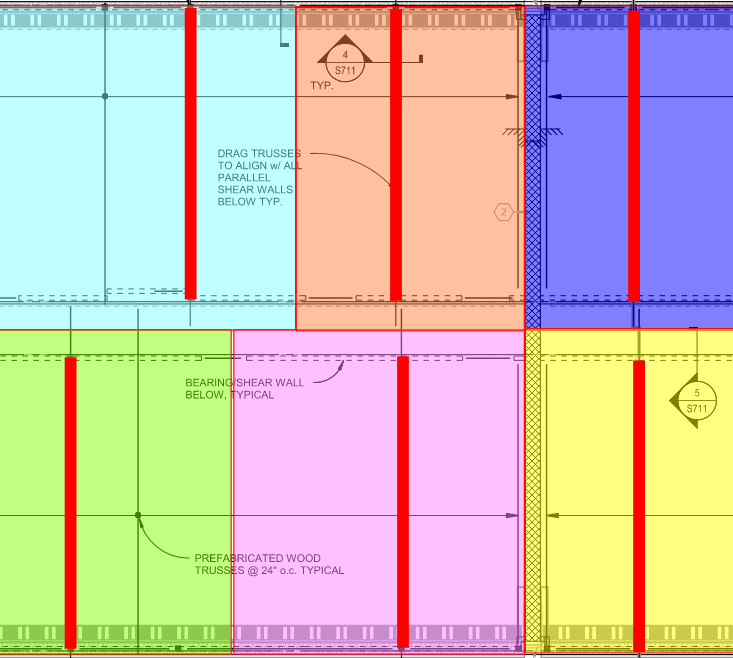
\includegraphics[width=0.6\linewidth,height=\textheight,keepaspectratio,alt={Shear walls (thick red lines) in plan view with their (colored) tributary areas.}]{images/shear_wall_tributary_area.png}
\caption{Shear walls (thick red lines) in plan view with their (colored)
tributary areas.}\label{fig:diaphragm_trib_area}
\end{figure}

    Shear wall shear forces are tabulated in
\autoref{tab:shear_wall_forces_roof_ns},
\autoref{tab:shear_wall_forces_level4_ns},
\autoref{tab:shear_wall_forces_level3_ns}, and
\autoref{tab:shear_wall_forces_level2_ns}.

Shear wall sheathing will be assumed to have the following properties:

\begin{enumerate}
\def\labelenumi{\arabic{enumi}.}
\tightlist
\item
  15/32'' thickness
\item
  10d common nails
\item
  Plywood panels
\item
  Sheathed on 1 side
\end{enumerate}

Notes:

\begin{itemize}
\tightlist
\item
  Cumulative shear force, \(F_{x,cum}\), is cumulative from the Roof
  downwards. For example, Level 3 includes the shear forces from the
  Roof, Level 4, and Level 3.
\end{itemize}

    \paragraph{Check aspect ratios}\label{check-aspect-ratios}

We must check the aspect ratios of the shear walls to ensure we don't
need to apply the aspect ratio factor in SDPWS Sec. 4.3.3.2. The maximum
aspect ratio of all N-S walls is:

    \begin{equation*}
\begin{aligned}
\mathrm{ratio}_{max} &= 0.575 \lt 2 \quad \textbf{\color{OK}OK}\ {\color{OK}\checkmark} \; 
\end{aligned}
\end{equation*}

    
    \(\therefore\) All aspect ratios are OK

    \begin{table}[H]
\centering
\caption{Shear wall forces NS - Roof}
\label{tab:shear_wall_forces_roof_ns}
\begin{tabular}{lrrrrrrrrr}
\toprule
 & $w_{trib}$ [psf] & $A$ [ft$^2$] & $F_x$ [lbf] & $F_{x,cum}$ [lbf] & $l_{wall}$ [ft] & $v$ [plf] & $0.7 v$ [lbf] & $v_{cap}$ [plf] & $s_{nail}$ [in] \\
Wall &  &  &  &  &  &  &  &  &  \\
\midrule
A-2 & 4.63 & 1662 & 7693 & 7693 & 30.8 & 250 & 175 & 311 & 6.00 \\
A-2.4 & 4.63 & 2147 & 9934 & 9934 & 30.8 & 323 & 226 & 311 & 6.00 \\
A-3.7 & 4.63 & 741 & 3430 & 3430 & 20.0 & 171 & 120 & 311 & 6.00 \\
A-4 & 4.63 & 505 & 2338 & 2338 & 20.0 & 117 & 81.8 & 311 & 6.00 \\
A-5 & 4.63 & 771 & 3565 & 3565 & 30.8 & 116 & 81.2 & 311 & 6.00 \\
A-5.1 & 4.63 & 1385 & 6407 & 6407 & 30.8 & 208 & 146 & 311 & 6.00 \\
A-6 & 4.63 & 988 & 4573 & 4573 & 30.8 & 149 & 104 & 311 & 6.00 \\
A-6.1 & 4.63 & 826 & 3824 & 3824 & 30.8 & 124 & 87.0 & 311 & 6.00 \\
A-6.8 & 4.63 & 906 & 4192 & 4192 & 30.8 & 136 & 95.4 & 311 & 6.00 \\
A-7 & 4.63 & 1012 & 4683 & 4683 & 30.8 & 152 & 107 & 311 & 6.00 \\
A-7.8 & 4.63 & 641 & 2965 & 2965 & 20.0 & 148 & 104 & 311 & 6.00 \\
A-8 & 4.63 & 794 & 3675 & 3675 & 30.8 & 120 & 83.7 & 311 & 6.00 \\
A-8.2 & 4.63 & 448 & 2073 & 2073 & 20.0 & 104 & 72.6 & 311 & 6.00 \\
A-8.9 & 4.63 & 1353 & 6259 & 6259 & 30.8 & 204 & 142 & 311 & 6.00 \\
A-9 & 4.63 & 1231 & 5697 & 5697 & 30.8 & 185 & 130 & 311 & 6.00 \\
\bottomrule
\end{tabular}
\end{table}


    
    \begin{table}[H]
\centering
\caption{Shear wall forces NS - Level 4}
\label{tab:shear_wall_forces_level4_ns}
\begin{tabular}{lrrrrrrrrr}
\toprule
 & $w_{trib}$ [psf] & $A$ [ft$^2$] & $F_x$ [lbf] & $F_{x,cum}$ [lbf] & $l_{wall}$ [ft] & $v$ [plf] & $0.7 v$ [lbf] & $v_{cap}$ [plf] & $s_{nail}$ [in] \\
Wall &  &  &  &  &  &  &  &  &  \\
\midrule
A-2 & 4.56 & 1662 & 7578 & 15270 & 30.8 & 497 & 348 & 461 & 4.00 \\
A-2.4 & 4.56 & 2147 & 9785 & 19719 & 30.8 & 641 & 449 & 461 & 4.00 \\
A-3.7 & 4.56 & 741 & 3378 & 6808 & 20.0 & 340 & 238 & 311 & 6.00 \\
A-4 & 4.56 & 505 & 2303 & 4641 & 20.0 & 232 & 162 & 311 & 6.00 \\
A-5 & 4.56 & 771 & 3512 & 7077 & 30.8 & 230 & 161 & 311 & 6.00 \\
A-5.1 & 4.56 & 1385 & 6311 & 12719 & 30.8 & 414 & 290 & 311 & 6.00 \\
A-6 & 4.56 & 988 & 4505 & 9078 & 30.8 & 295 & 207 & 311 & 6.00 \\
A-6.1 & 4.56 & 826 & 3766 & 7590 & 30.8 & 247 & 173 & 311 & 6.00 \\
A-6.8 & 4.56 & 906 & 4129 & 8321 & 30.8 & 271 & 189 & 311 & 6.00 \\
A-7 & 4.56 & 1012 & 4613 & 9296 & 30.8 & 302 & 212 & 311 & 6.00 \\
A-7.8 & 4.56 & 641 & 2920 & 5885 & 20.0 & 294 & 206 & 311 & 6.00 \\
A-8 & 4.56 & 794 & 3620 & 7295 & 30.8 & 237 & 166 & 311 & 6.00 \\
A-8.2 & 4.56 & 448 & 2042 & 4116 & 20.0 & 206 & 144 & 311 & 6.00 \\
A-8.9 & 4.56 & 1353 & 6165 & 12424 & 30.8 & 404 & 283 & 311 & 6.00 \\
A-9 & 4.56 & 1231 & 5612 & 11308 & 30.8 & 368 & 257 & 311 & 6.00 \\
\bottomrule
\end{tabular}
\end{table}


    
    \begin{table}[H]
\centering
\caption{Shear wall forces NS - Level 3}
\label{tab:shear_wall_forces_level3_ns}
\begin{tabular}{lrrrrrrrrr}
\toprule
 & $w_{trib}$ [psf] & $A$ [ft$^2$] & $F_x$ [lbf] & $F_{x,cum}$ [lbf] & $l_{wall}$ [ft] & $v$ [plf] & $0.7 v$ [lbf] & $v_{cap}$ [plf] & $s_{nail}$ [in] \\
Wall &  &  &  &  &  &  &  &  &  \\
\midrule
A-2 & 3.10 & 1662 & 5147 & 20417 & 30.8 & 664 & 465 & 600 & 3.00 \\
A-2.4 & 3.10 & 2147 & 6646 & 26365 & 30.8 & 857 & 600 & 770 & 2.00 \\
A-3.7 & 3.10 & 741 & 2295 & 9103 & 20.0 & 455 & 319 & 461 & 4.00 \\
A-4 & 3.10 & 505 & 1564 & 6206 & 20.0 & 310 & 217 & 311 & 6.00 \\
A-5 & 3.10 & 771 & 2385 & 9463 & 30.8 & 308 & 215 & 311 & 6.00 \\
A-5.1 & 3.10 & 1385 & 4287 & 17005 & 30.8 & 553 & 387 & 461 & 4.00 \\
A-6 & 3.10 & 988 & 3059 & 12137 & 30.8 & 395 & 276 & 311 & 6.00 \\
A-6.1 & 3.10 & 826 & 2558 & 10148 & 30.8 & 330 & 231 & 311 & 6.00 \\
A-6.8 & 3.10 & 906 & 2804 & 11126 & 30.8 & 362 & 253 & 311 & 6.00 \\
A-7 & 3.10 & 1012 & 3133 & 12428 & 30.8 & 404 & 283 & 311 & 6.00 \\
A-7.8 & 3.10 & 641 & 1983 & 7868 & 20.0 & 393 & 275 & 311 & 6.00 \\
A-8 & 3.10 & 794 & 2459 & 9754 & 30.8 & 317 & 222 & 311 & 6.00 \\
A-8.2 & 3.10 & 448 & 1387 & 5503 & 20.0 & 275 & 193 & 311 & 6.00 \\
A-8.9 & 3.10 & 1353 & 4187 & 16611 & 30.8 & 540 & 378 & 461 & 4.00 \\
A-9 & 3.10 & 1231 & 3811 & 15120 & 30.8 & 492 & 344 & 461 & 4.00 \\
\bottomrule
\end{tabular}
\end{table}


    
    \begin{table}[H]
\centering
\caption{Shear wall forces NS - Level 2}
\label{tab:shear_wall_forces_level2_ns}
\begin{tabular}{lrrrrrrrrr}
\toprule
 & $w_{trib}$ [psf] & $A$ [ft$^2$] & $F_x$ [lbf] & $F_{x,cum}$ [lbf] & $l_{wall}$ [ft] & $v$ [plf] & $0.7 v$ [lbf] & $v_{cap}$ [plf] & $s_{nail}$ [in] \\
Wall &  &  &  &  &  &  &  &  &  \\
\midrule
A-2 & 1.63 & 1662 & 2708 & 23125 & 30.8 & 752 & 526 & 600 & 3.00 \\
A-2.4 & 1.63 & 2147 & 3497 & 29862 & 30.8 & 971 & 680 & 770 & 2.00 \\
A-3.7 & 1.63 & 741 & 1207 & 10310 & 20.0 & 516 & 361 & 461 & 4.00 \\
A-4 & 1.63 & 505 & 823 & 7029 & 20.0 & 351 & 246 & 311 & 6.00 \\
A-5 & 1.63 & 771 & 1255 & 10718 & 30.8 & 349 & 244 & 311 & 6.00 \\
A-5.1 & 1.63 & 1385 & 2256 & 19261 & 30.8 & 626 & 438 & 461 & 4.00 \\
A-6 & 1.63 & 988 & 1610 & 13747 & 30.8 & 447 & 313 & 461 & 4.00 \\
A-6.1 & 1.63 & 826 & 1346 & 11495 & 30.8 & 374 & 262 & 311 & 6.00 \\
A-6.8 & 1.63 & 906 & 1476 & 12601 & 30.8 & 410 & 287 & 311 & 6.00 \\
A-7 & 1.63 & 1012 & 1649 & 14077 & 30.8 & 458 & 320 & 461 & 4.00 \\
A-7.8 & 1.63 & 641 & 1044 & 8912 & 20.0 & 446 & 312 & 461 & 4.00 \\
A-8 & 1.63 & 794 & 1294 & 11048 & 30.8 & 359 & 251 & 311 & 6.00 \\
A-8.2 & 1.63 & 448 & 730 & 6233 & 20.0 & 312 & 218 & 311 & 6.00 \\
A-8.9 & 1.63 & 1353 & 2203 & 18814 & 30.8 & 612 & 428 & 461 & 4.00 \\
A-9 & 1.63 & 1231 & 2006 & 17125 & 30.8 & 557 & 390 & 461 & 4.00 \\
\bottomrule
\end{tabular}
\end{table}


    
    \paragraph{East-West Direction}\label{east-west-direction}

    Most likely, the shear walls in the E-W direction will be governed by a
rigid diaphragm assumption.

    Shear wall shear forces are tabulated in
\autoref{tab:shear_wall_forces_roof_ew},
\autoref{tab:shear_wall_forces_level4_ew},
\autoref{tab:shear_wall_forces_level3_ew}, and
\autoref{tab:shear_wall_forces_level2_ew}.\\

    \paragraph{Check aspect ratios}\label{check-aspect-ratios}

We will also check the aspect ratios of the E-W walls.

    \begin{equation*}
\begin{aligned}
\mathrm{ratio}_{max} &= 1.7 \lt 2 \quad \textbf{\color{OK}OK}\ {\color{OK}\checkmark} \; 
\end{aligned}
\end{equation*}

    
    \(\therefore\) All aspect ratios are OK

    \begin{Verbatim}[commandchars=\\\{\}]
C:\textbackslash{}Users\textbackslash{}Andy.Sazima\textbackslash{}AppData\textbackslash{}Local\textbackslash{}Temp\textbackslash{}ipykernel\_41468\textbackslash{}312644044.py:16:
UserWarning: The following walls have insufficient capacity:
                      DCR  adjusted shear demand  adjusted shear capacity  \textbackslash{}
Level   Wall
Level 3 A-C.7.5  1.053286             810.653887               769.642857
Level 2 A-C.1.8  1.081066             832.035106               769.642857
        A-C.7.5  1.192995             918.180155               769.642857

                 nail spacing
Level   Wall
Level 3 A-C.7.5           2.0
Level 2 A-C.1.8           2.0
        A-C.7.5           2.0
  warnings.warn(
    \end{Verbatim}

    \begin{table}[H]
\centering
\caption{Shear wall forces EW - Roof}
\label{tab:shear_wall_forces_roof_ew}
\begin{tabular}{lrrrrrrrrrr}
\toprule
 & $w_{trib}$ [psf] & $A$ [ft$^2$] & $F_x$ [lbf] & $F_{x,cum}$ [lbf] & $l_{wall}$ [ft] & $v$ [plf] & $0.7 v$ [lbf] & $v_{cap}$ [plf] & $s_{nail}$ [in] & DCR \\
Wall &  &  &  &  &  &  &  &  &  &  \\
\midrule
A-B.1 & 4.63 & 1131 & 5232 & 5232 & 26.0 & 201 & 141 & 311 & 6.00 & 0.453 \\
A-B.2.5 & 4.63 & 745 & 3449 & 3449 & 13.2 & 260 & 182 & 311 & 6.00 & 0.586 \\
A-B.3.5 & 4.63 & 536 & 2480 & 2480 & 9.00 & 276 & 193 & 311 & 6.00 & 0.621 \\
A-B.4 & 4.63 & 636 & 2945 & 2945 & 12.0 & 245 & 172 & 311 & 6.00 & 0.553 \\
A-B.4.8 & 4.63 & 536 & 2480 & 2480 & 11.0 & 225 & 158 & 311 & 6.00 & 0.508 \\
A-B.5.5 & 4.63 & 1156 & 5348 & 5348 & 29.8 & 180 & 126 & 311 & 6.00 & 0.405 \\
A-B.6.5 & 4.63 & 946 & 4379 & 4379 & 12.8 & 343 & 240 & 311 & 6.00 & 0.774 \\
A-B.7.9 & 4.63 & 955 & 4418 & 4418 & 16.2 & 272 & 190 & 311 & 6.00 & 0.613 \\
A-B.8.8 & 4.63 & 1064 & 4922 & 4922 & 13.8 & 358 & 251 & 311 & 6.00 & 0.806 \\
A-C.1.8 & 4.63 & 1474 & 6821 & 6821 & 17.2 & 395 & 277 & 311 & 6.00 & 0.891 \\
A-C.3.2 & 4.63 & 1038 & 4806 & 4806 & 23.0 & 209 & 146 & 311 & 6.00 & 0.471 \\
A-C.4.2 & 4.63 & 921 & 4263 & 4263 & 22.5 & 189 & 133 & 311 & 6.00 & 0.427 \\
A-C.5.5 & 4.63 & 1038 & 4806 & 4806 & 26.0 & 185 & 129 & 311 & 6.00 & 0.416 \\
A-C.6.5 & 4.63 & 519 & 2403 & 2403 & 11.2 & 214 & 150 & 311 & 6.00 & 0.481 \\
A-C.6.9 & 4.63 & 413 & 1913 & 1913 & 7.00 & 273 & 191 & 311 & 6.00 & 0.616 \\
A-C.7.5 & 4.63 & 636 & 2945 & 2945 & 6.75 & 436 & 305 & 311 & 6.00 & 0.983 \\
A-C.8.5 & 4.63 & 715 & 3307 & 3307 & 10.2 & 323 & 226 & 311 & 6.00 & 0.727 \\
A-C.9.2 & 4.63 & 949 & 4392 & 4392 & 25.2 & 174 & 122 & 311 & 6.00 & 0.392 \\
\bottomrule
\end{tabular}
\end{table}


    
    \begin{table}[H]
\centering
\caption{Shear wall forces EW - Level 4}
\label{tab:shear_wall_forces_level4_ew}
\begin{tabular}{lrrrrrrrrrr}
\toprule
 & $w_{trib}$ [psf] & $A$ [ft$^2$] & $F_x$ [lbf] & $F_{x,cum}$ [lbf] & $l_{wall}$ [ft] & $v$ [plf] & $0.7 v$ [lbf] & $v_{cap}$ [plf] & $s_{nail}$ [in] & DCR \\
Wall &  &  &  &  &  &  &  &  &  &  \\
\midrule
A-B.1 & 4.56 & 1131 & 5153 & 10385 & 26.0 & 399 & 280 & 311 & 6.00 & 0.900 \\
A-B.2.5 & 4.56 & 745 & 3397 & 6847 & 13.2 & 517 & 362 & 461 & 4.00 & 0.785 \\
A-B.3.5 & 4.56 & 536 & 2443 & 4923 & 9.00 & 547 & 383 & 461 & 4.00 & 0.831 \\
A-B.4 & 4.56 & 636 & 2901 & 5847 & 12.0 & 487 & 341 & 461 & 4.00 & 0.740 \\
A-B.4.8 & 4.56 & 536 & 2443 & 4923 & 11.0 & 448 & 313 & 461 & 4.00 & 0.680 \\
A-B.5.5 & 4.56 & 1156 & 5268 & 10616 & 29.8 & 357 & 250 & 311 & 6.00 & 0.804 \\
A-B.6.5 & 4.56 & 946 & 4314 & 8693 & 12.8 & 682 & 477 & 600 & 3.00 & 0.795 \\
A-B.7.9 & 4.56 & 955 & 4352 & 8770 & 16.2 & 540 & 378 & 461 & 4.00 & 0.820 \\
A-B.8.8 & 4.56 & 1064 & 4848 & 9770 & 13.8 & 711 & 497 & 600 & 3.00 & 0.829 \\
A-C.1.8 & 4.56 & 1474 & 6719 & 13539 & 17.2 & 785 & 549 & 600 & 3.00 & 0.916 \\
A-C.3.2 & 4.56 & 1038 & 4734 & 9539 & 23.0 & 415 & 290 & 311 & 6.00 & 0.934 \\
A-C.4.2 & 4.56 & 921 & 4199 & 8462 & 22.5 & 376 & 263 & 311 & 6.00 & 0.847 \\
A-C.5.5 & 4.56 & 1038 & 4734 & 9539 & 26.0 & 367 & 257 & 311 & 6.00 & 0.827 \\
A-C.6.5 & 4.56 & 519 & 2367 & 4770 & 11.2 & 424 & 297 & 311 & 6.00 & 0.955 \\
A-C.6.9 & 4.56 & 413 & 1884 & 3797 & 7.00 & 542 & 380 & 461 & 4.00 & 0.824 \\
A-C.7.5 & 4.56 & 636 & 2901 & 5847 & 6.75 & 866 & 606 & 770 & 2.00 & 0.788 \\
A-C.8.5 & 4.56 & 715 & 3257 & 6564 & 10.2 & 640 & 448 & 461 & 4.00 & 0.973 \\
A-C.9.2 & 4.56 & 949 & 4326 & 8718 & 25.2 & 345 & 242 & 311 & 6.00 & 0.778 \\
\bottomrule
\end{tabular}
\end{table}


    
    \begin{table}[H]
\centering
\caption{Shear wall forces EW - Level 3}
\label{tab:shear_wall_forces_level3_ew}
\begin{tabular}{lrrrrrrrrrr}
\toprule
 & $w_{trib}$ [psf] & $A$ [ft$^2$] & $F_x$ [lbf] & $F_{x,cum}$ [lbf] & $l_{wall}$ [ft] & $v$ [plf] & $0.7 v$ [lbf] & $v_{cap}$ [plf] & $s_{nail}$ [in] & DCR \\
Wall &  &  &  &  &  &  &  &  &  &  \\
\midrule
A-B.1 & 3.10 & 1131 & 3500 & 13885 & 26.0 & 534 & 374 & 461 & 4.00 & 0.811 \\
A-B.2.5 & 3.10 & 745 & 2308 & 9154 & 13.2 & 691 & 484 & 600 & 3.00 & 0.806 \\
A-B.3.5 & 3.10 & 536 & 1659 & 6583 & 9.00 & 731 & 512 & 600 & 3.00 & 0.853 \\
A-B.4 & 3.10 & 636 & 1970 & 7817 & 12.0 & 651 & 456 & 461 & 4.00 & 0.990 \\
A-B.4.8 & 3.10 & 536 & 1659 & 6583 & 11.0 & 598 & 419 & 461 & 4.00 & 0.909 \\
A-B.5.5 & 3.10 & 1156 & 3578 & 14194 & 29.8 & 477 & 334 & 461 & 4.00 & 0.725 \\
A-B.6.5 & 3.10 & 946 & 2930 & 11623 & 12.8 & 912 & 638 & 770 & 2.00 & 0.829 \\
A-B.7.9 & 3.10 & 955 & 2956 & 11726 & 16.2 & 722 & 505 & 600 & 3.00 & 0.842 \\
A-B.8.8 & 3.10 & 1064 & 3293 & 13063 & 13.8 & 950 & 665 & 770 & 2.00 & 0.864 \\
A-C.1.8 & 3.10 & 1474 & 4563 & 18103 & 17.2 & 1049 & 735 & 770 & 2.00 & 0.954 \\
A-C.3.2 & 3.10 & 1038 & 3215 & 12754 & 23.0 & 555 & 388 & 461 & 4.00 & 0.843 \\
A-C.4.2 & 3.10 & 921 & 2852 & 11314 & 22.5 & 503 & 352 & 461 & 4.00 & 0.764 \\
A-C.5.5 & 3.10 & 1038 & 3215 & 12754 & 26.0 & 491 & 343 & 461 & 4.00 & 0.745 \\
A-C.6.5 & 3.10 & 519 & 1607 & 6377 & 11.2 & 567 & 397 & 461 & 4.00 & 0.861 \\
A-C.6.9 & 3.10 & 413 & 1280 & 5077 & 7.00 & 725 & 508 & 600 & 3.00 & 0.846 \\
A-C.7.5 & {\cellcolor{yellow}} 3.10 & {\cellcolor{yellow}} 636 & {\cellcolor{yellow}} 1970 & {\cellcolor{yellow}} 7817 & {\cellcolor{yellow}} 6.75 & {\cellcolor{yellow}} 1158 & {\cellcolor{yellow}} 811 & {\cellcolor{yellow}} 770 & {\cellcolor{yellow}} 2.00 & {\cellcolor{yellow}} 1.05 \\
A-C.8.5 & 3.10 & 715 & 2212 & 8776 & 10.2 & 856 & 599 & 600 & 3.00 & 0.999 \\
A-C.9.2 & 3.10 & 949 & 2938 & 11656 & 25.2 & 462 & 323 & 461 & 4.00 & 0.701 \\
\bottomrule
\end{tabular}
\end{table}


    
    \begin{table}[H]
\centering
\caption{Shear wall forces EW - Level 2}
\label{tab:shear_wall_forces_level2_ew}
\begin{tabular}{lrrrrrrrrrr}
\toprule
 & $w_{trib}$ [psf] & $A$ [ft$^2$] & $F_x$ [lbf] & $F_{x,cum}$ [lbf] & $l_{wall}$ [ft] & $v$ [plf] & $0.7 v$ [lbf] & $v_{cap}$ [plf] & $s_{nail}$ [in] & DCR \\
Wall &  &  &  &  &  &  &  &  &  &  \\
\midrule
A-B.1 & 1.63 & 1131 & 1842 & 15727 & 26.0 & 605 & 423 & 461 & 4.00 & 0.919 \\
A-B.2.5 & 1.63 & 745 & 1214 & 10368 & 13.2 & 783 & 548 & 600 & 3.00 & 0.913 \\
A-B.3.5 & 1.63 & 536 & 873 & 7456 & 9.00 & 828 & 580 & 600 & 3.00 & 0.967 \\
A-B.4 & 1.63 & 636 & 1037 & 8854 & 12.0 & 738 & 516 & 600 & 3.00 & 0.861 \\
A-B.4.8 & 1.63 & 536 & 873 & 7456 & 11.0 & 678 & 474 & 600 & 3.00 & 0.791 \\
A-B.5.5 & 1.63 & 1156 & 1883 & 16077 & 29.8 & 540 & 378 & 461 & 4.00 & 0.821 \\
A-B.6.5 & 1.63 & 946 & 1542 & 13164 & 12.8 & 1032 & 723 & 770 & 2.00 & 0.939 \\
A-B.7.9 & 1.63 & 955 & 1555 & 13281 & 16.2 & 817 & 572 & 600 & 3.00 & 0.953 \\
A-B.8.8 & 1.63 & 1064 & 1733 & 14795 & 13.8 & 1076 & 753 & 770 & 2.00 & 0.979 \\
A-C.1.8 & {\cellcolor{yellow}} 1.63 & {\cellcolor{yellow}} 1474 & {\cellcolor{yellow}} 2401 & {\cellcolor{yellow}} 20504 & {\cellcolor{yellow}} 17.2 & {\cellcolor{yellow}} 1189 & {\cellcolor{yellow}} 832 & {\cellcolor{yellow}} 770 & {\cellcolor{yellow}} 2.00 & {\cellcolor{yellow}} 1.08 \\
A-C.3.2 & 1.63 & 1038 & 1692 & 14446 & 23.0 & 628 & 440 & 461 & 4.00 & 0.954 \\
A-C.4.2 & 1.63 & 921 & 1501 & 12815 & 22.5 & 570 & 399 & 461 & 4.00 & 0.865 \\
A-C.5.5 & 1.63 & 1038 & 1692 & 14446 & 26.0 & 556 & 389 & 461 & 4.00 & 0.844 \\
A-C.6.5 & 1.63 & 519 & 846 & 7223 & 11.2 & 642 & 449 & 461 & 4.00 & 0.975 \\
A-C.6.9 & 1.63 & 413 & 673 & 5750 & 7.00 & 821 & 575 & 600 & 3.00 & 0.958 \\
A-C.7.5 & {\cellcolor{yellow}} 1.63 & {\cellcolor{yellow}} 636 & {\cellcolor{yellow}} 1037 & {\cellcolor{yellow}} 8854 & {\cellcolor{yellow}} 6.75 & {\cellcolor{yellow}} 1312 & {\cellcolor{yellow}} 918 & {\cellcolor{yellow}} 770 & {\cellcolor{yellow}} 2.00 & {\cellcolor{yellow}} 1.19 \\
A-C.8.5 & 1.63 & 715 & 1164 & 9940 & 10.2 & 970 & 679 & 770 & 2.00 & 0.882 \\
A-C.9.2 & 1.63 & 949 & 1546 & 13202 & 25.2 & 523 & 366 & 461 & 4.00 & 0.794 \\
\bottomrule
\end{tabular}
\end{table}


    
    \subsubsection{Rigid Diaphragm
Assumption}\label{rigid-diaphragm-assumption}

    With a rigid diaphragm assumption, we now must calculate in each
direction:

\begin{enumerate}
\def\labelenumi{\arabic{enumi}.}
\tightlist
\item
  The relative stiffnesses of the shear walls to obtain a center of
  rigidity.
\item
  The center of mass of the diaphragm with the center of rigidity to
  obtain an eccentricity.
\end{enumerate}

The relative stiffnesses of the shear walls can be calculated by using
the deflection equation from NDS SDPWS Sec. 4.3.4

\begin{align*}
k &= \frac{F}{\delta},\, \text{assume }F = 1 \\
\delta_{sw} &= \frac{8vh^3}{EAb} + \frac{vh}{1000 G_a} + \frac{h \Delta_A}{b}\quad \text{(SDPWS Eq. 4.3-1)}
\end{align*}

where

\begin{itemize}
\tightlist
\item
  \(b =\) the shear wall length {[}ft{]}
\item
  \(\Delta_A =\) vertical deformation of the wall overturning anchorage
  system + vertical compression deformation {[}in{]}
\item
  \(E =\) modulus of elasticity of end posts {[}psi{]}
\item
  \(A =\) area of end post cross-section {[}in\(^2\){]}
\item
  \(G_a =\) apparent shear wall shear stiffness from nail slip and panel
  shear deformation {[}kip/in{]}
\item
  \(h =\) shear wall height {[}ft{]}
\item
  \(v =\) unit shear force induced by the design load {[}plf{]}
\item
  \(\delta_{sw} =\) maximum shear wall deflection determined by elastic
  analysis {[}in{]}
\end{itemize}

We will assume that the end posts are (2) 2x4 Douglas Fir No.~2; this
means:

    \begin{equation*}
\begin{aligned}
E_{endpost} &= 1.6e+06\ \mathrm{psi} \; 
\\
A_{endpost} &= 2 \cdot 5.25 \cdot \left( \mathrm{inch} \right) ^{ 2 }  = 2 \cdot 5.25 \cdot \left( inch \right) ^{ 2 } &= 10.5\ \mathrm{inch}^{2}  
\end{aligned}
\end{equation*}

    
    We will assume a continuous tiedown rod system. A conservative
first-pass value for \(\Delta_A\) can be:

    \begin{equation*}
\begin{aligned}
\Delta_{A} &= 0.25 \cdot \mathrm{inch}  = 0.25 \cdot inch &= 0.25\ \mathrm{inch}  
\end{aligned}
\end{equation*}

    
    \subparagraph{Story Drift}\label{story-drift}

We can check the story drift at each shear wall line. This is
conservative but all-encompassing.

First, we start with the total deflection at level \(x\), \(\delta_x\):

\[
\delta_x = \frac{C_d \delta_{xe}}{I_e}\quad \text{(ASCE 7-16 Eq. 12.8-15)}
\]

The total displacement needs to be converted to per-story displacement,
but the shear wall displacement, \(\delta_{sw}\), is already per story,
so the story drift, \(\Delta_x\), is:

\[
\Delta_x = \frac{C_d \delta_{sw,x}}{I_e}
\]

The story drift can't exceed the allowable story drift, \(\Delta_a\),
which is defined in ASCE 7-16 Table 12.12-1. In our case:

\begin{itemize}
\tightlist
\item
  Structure is not masonry shear wall
\item
  Four stories or less above the base
\item
  Interior walls, partitions, ceilings, and exterior wall systems are
  designed to accommodate story drifts.
\end{itemize}

Therefore:

\[
\Delta_a = 0.025 h_{sx}
\]

where \(h_{sx}\) is the story height below level \(x\).

    The ratio of the story drift, \(\Delta_x\), and the the maximum story
drift, \(\Delta_a\), must not exceed 1

\[
\text{ratio}_{drift} = \frac{\Delta_x}{\Delta_a} \leq 1
\]

    \begin{equation*}
\begin{aligned}
\mathrm{ratio}_{drift,max} &= 1.417 \; 
\\
check_{\Delta} &= 1.42 \gt 1 \quad \textbf{{\color{NG}NG !}} \; 
\end{aligned}
\end{equation*}

    
    \subparagraph{Shear Wall Rigidities}\label{shear-wall-rigidities}

With the deflections of each shear wall, along with the force demand of
each shear wall, we can obtain the stiffnesses (and therefore, relative
stiffnesses) of all the walls.

\[
k = \frac{F_x}{\delta_{sw}}
\]

            \begin{tcolorbox}[breakable, size=fbox, boxrule=.5pt, pad at break*=1mm, opacityfill=0]
\begin{Verbatim}[commandchars=\\\{\}]
                Direction   unit shear  wall length  wall height  \textbackslash{}
Level   Wall
Roof    A-B.1         E-W   201.226548        26.00         10.0
        A-B.2.5       E-W   260.314874        13.25         10.0
        A-B.3.5       E-W   275.589280         9.00         10.0
        A-B.4         E-W   245.446702        12.00         10.0
        A-B.4.8       E-W   225.482138        11.00         10.0
{\ldots}                   {\ldots}          {\ldots}          {\ldots}          {\ldots}
Level 2 A-C.6.5       E-W   642.035747        11.25         11.5
        A-C.6.9       E-W   821.480301         7.00         11.5
        A-C.7.5       E-W  1311.685936         6.75         11.5
        A-C.8.5       E-W   969.721498        10.25         11.5
        A-C.9.2       E-W   522.835690        25.25         11.5

                 shear stiffness  nail spacing  end post youngs modulus  \textbackslash{}
Level   Wall
Roof    A-B.1               14.0           6.0                1600000.0
        A-B.2.5             14.0           6.0                1600000.0
        A-B.3.5             14.0           6.0                1600000.0
        A-B.4               14.0           6.0                1600000.0
        A-B.4.8             14.0           6.0                1600000.0
{\ldots}                          {\ldots}           {\ldots}                      {\ldots}
Level 2 A-C.6.5             17.0           4.0                1600000.0
        A-C.6.9             19.0           3.0                1600000.0
        A-C.7.5             23.0           2.0                1600000.0
        A-C.8.5             23.0           2.0                1600000.0
        A-C.9.2             17.0           4.0                1600000.0

                 end post area  Delta\_A  delta\_sw  story drift  Delta\_a  \textbackslash{}
Level   Wall
Roof    A-B.1             10.5     0.25  0.243573     0.974290     3.00
        A-B.2.5           10.5     0.25  0.383974     1.535895     3.00
        A-B.3.5           10.5     0.25  0.489209     1.956835     3.00
        A-B.4             10.5     0.25  0.393392     1.573569     3.00
        A-B.4.8           10.5     0.25  0.398093     1.592370     3.00
{\ldots}                        {\ldots}      {\ldots}       {\ldots}          {\ldots}      {\ldots}
Level 2 A-C.6.5           10.5     0.25  0.731205     2.924821     3.45
        A-C.6.9           10.5     0.25  0.992917     3.971669     3.45
        A-C.7.5           10.5     0.25  1.222503     4.890013     3.45
        A-C.8.5           10.5     0.25  0.833865     3.335462     3.45
        A-C.9.2           10.5     0.25  0.482540     1.930162     3.45

                 story drift check  story drift dcr  cumulative shear  \textbackslash{}
Level   Wall
Roof    A-B.1                 True         0.324763       5231.890237
        A-B.2.5               True         0.511965       3449.172082
        A-B.3.5               True         0.652278       2480.303520
        A-B.4                 True         0.524523       2945.360430
        A-B.4.8               True         0.530790       2480.303520
{\ldots}                            {\ldots}              {\ldots}               {\ldots}
Level 2 A-C.6.5               True         0.847774       7222.902159
        A-C.6.9              False         1.151208       5750.362106
        A-C.7.5              False         1.417395       8853.880066
        A-C.8.5               True         0.966800       9939.645358
        A-C.9.2               True         0.559467      13201.601172

                 wall stiffness  total level stiffness  \textbackslash{}
Level   Wall
Roof    A-B.1      21479.801284          218627.090446
        A-B.2.5     8982.830163          218627.090446
        A-B.3.5     5070.031430          218627.090446
        A-B.4       7487.081007          218627.090446
        A-B.4.8     6230.469903          218627.090446
{\ldots}                         {\ldots}                    {\ldots}
Level 2 A-C.6.5     9878.076446          327538.879675
        A-C.6.9     5791.381738          327538.879675
        A-C.7.5     7242.418074          327538.879675
        A-C.8.5    11919.963722          327538.879675
        A-C.9.2    27358.538205          327538.879675

                 total level cumulative shear  relative wall stiffness  \textbackslash{}
Level   Wall
Roof    A-B.1                    71308.726197                 0.098249
        A-B.2.5                  71308.726197                 0.041087
        A-B.3.5                  71308.726197                 0.023190
        A-B.4                    71308.726197                 0.034246
        A-B.4.8                  71308.726197                 0.028498
{\ldots}                                       {\ldots}                      {\ldots}
Level 2 A-C.6.5                 214357.096337                 0.030158
        A-C.6.9                 214357.096337                 0.017682
        A-C.7.5                 214357.096337                 0.022112
        A-C.8.5                 214357.096337                 0.036393
        A-C.9.2                 214357.096337                 0.083528

                 direct shear force
Level   Wall
Roof    A-B.1           7005.981123
        A-B.2.5         2929.893891
        A-B.3.5         1653.671932
        A-B.4           2442.031353
        A-B.4.8         2032.167521
{\ldots}                             {\ldots}
Level 2 A-C.6.5         6464.685311
        A-C.6.9         3790.156986
        A-C.7.5         4739.784511
        A-C.8.5         7800.993929
        A-C.9.2        17904.734899

[72 rows x 20 columns]
\end{Verbatim}
\end{tcolorbox}
        

    % Add a bibliography block to the postdoc
    
    
    
\end{document}
